
%(BEGIN_QUESTION)
% Copyright 2006, Tony R. Kuphaldt, released under the Creative Commons Attribution License (v 1.0)
% This means you may do almost anything with this work of mine, so long as you give me proper credit

\vbox{\hrule \hbox{\strut \vrule{} $\int f(x) \> dx$ \hskip 5pt {\sl Calculus alert!} \vrule} \hrule}

Imagine a scenario where we are measuring municipal water flow through a pipe, using a turbine meter:

$$\includegraphics[width=15.5cm]{i00543x01.eps}$$

Suppose the municipality management decides they need a running total of water {\it volume} as well as water flow.  In other words, they want a counter that tallies up the number of gallons passed through this flowmeter.  An operator will record this total volume at the end of every day and then re-set the counter for the next day's tally.

Two instrument technicians have different ideas about how to do this.  One technician says it would be easy to electronically {\it integrate} the 4-20 mA flow signal to obtain a volume signal, while the other technician advocates a scheme to directly intercept the turbine's ``pick-up'' unit signal rather than the 4-20 mA flow signal and send that pulse signal to a digital counter.

Elaborate on these two technicians' plans, and then cast your own vote either for one of these plans or for an entirely different idea.

\underbar{file i00543}
%(END_QUESTION)





%(BEGIN_ANSWER)

The calculus operation of {\it time-integration} mathematically ``un-does'' differentiation.  If we know that flow is nothing more than rate of change of volume with respect to time, an ``integrator'' circuit should be able to un-do the flow signal to arrive at a volume signal:

$$Q = {dV \over dt} \hbox{\hskip 30pt Flow is the time-derivative of Volume}$$

$$V = \int^T_0 Q \> dt \hbox{\hskip 30pt Volume is the time-integral of Flow}$$

A simple analog circuit to perform the time-integral function is shown here:

$$\includegraphics[width=15.5cm]{i00543x02.eps}$$

$$V_{out} = - {1 \over {RC}} \int^T_0 V_{in} \> dt$$

Of course, we would have to add a lot of extra parts to this circuit to get it ready to receive a 4-20 mA signal in!  It should be noted that integration over long time periods is almost always done digitally, due to the problems of drift associated with analog circuitry.

\vskip 10pt

The second technician's idea -- to clock a digital counter circuit off the turbine meter's pulse output -- would be easier (a simpler circuit) and more practical (less to calibrate).

%(END_ANSWER)





%(BEGIN_NOTES)


%INDEX% Measurement, flow: totalizer

%(END_NOTES)


